
%\chapter{Tests and Results}
 \chapter{Teste și rezultate experimentale}
\label{cap:rezultate}

%Ponderea acestui capitol relativ la întreaga lucrare este de 5-10\%.
%
%Aici sunt prezentate metodele de validare a soluțiilor/sistemului descris în capitolele anterioare, scenariile de testare a corectitudinii funcționale, a utilizabilității, performanței etc.   
%
%Rezultatele testelor experimentale necesită, în general interpretări (dacă rezultatele obținute corespund așteptărilor, intuițiilor cititorului, de ce apar variații/excepții etc.) și comparații cu rezultatele altor metode similare. 
%
%Sistemele de testare și testele propriu-zise trebuie descrise detaliat astfel încât să poată fi reproduse și de alții care poate vor să-și compare soluțiile lor cu a voastră (eventual, codul testelor poate fi pus în anexe). Dacă se poate alegeți pentru evaluarea sistemului vostru benchmark-uri (pachete de testare) dedicate, astfel încât comparația cu alte sisteme să poată fi făcută mai ușor. În plus, astfel de teste sunt mult mai complete și mai realiste decât cele dezvoltate de voi. Oricum, încercați ca testele efectuate să nu fie triviale, ci să acopere scenarii cât mai reale, mai complexe și mai relevante ale funcționării sistemului vostru. 

%\section{Functional Tests}
 \section{Teste de funcționalitate}
 
 In testarea sistemului s-a pus accentul pe testare celor doua functionalitati de protectie impotriva atacurilor de SQL injection si a utilizatorilor de Tor.
 
 Pentru testarea modelului folosit in prevenirea atacurilor de SQL injection s-a folosit setul de date de test specificat si in capitolul 6. Acest set a fost obtinut din setul initial de date de antrenare, acesta fiind impartit in 2 seturi separate cu proportia de 70\%(set antrenaere) si respectiv 30\%(set testare).
 
\begin{center}
	\begin{tabular}{||c c c c||} 
		\hline
		Tip set de testare  & Preziceri corecte & Dimensiune set & Acuratete(\%) \\ [0.5ex] 
		\hline\hline
		Clean \& infected & 187596 & 189278 & 99.11 \\ 
		\hline
		Clean & 5466 & 6258 & 87.34 \\
		\hline
		Infected & 182130 & 193020 & 99.51 \\
		\hline
	\end{tabular}
\end{center}

Pe baza tabelului de mai sus se pot observa diferente majore de porformanta intre detectia pe setul "Clean" si pe "Infected". Aceste diferente, respectiv scaderi de performanta in cazul setului Clean, se datoreaza dimensiunii mult mai mici a setuli de Clean folosit si in antrenarea modelului.

Pentru testarea eficientei sistemului de blocare a adreselor IP ale retelei Tor, s-a realizat o referinta intre datele colectate de modulul de monitorizare a activitatii retelei Tor.

In prima diagrama este prezentata diferenta procentuala dintre adresele IP cu un uptime mai mare de 7 zile in ultima luna si cele cu un uptime mai mic. In cea de a doua diagrama este evidentiata diferenta dintre uptime-ul total ale acestor adrese IP din ultima luna. Printr-o analiza simpla in paralel a datelor din cele doua diagrame, se poate observa ca desi doar 20.31\% din IP urile folosite de reteaua Tor sunt bloacate, din timpul total de uptime din ultima luna, 75.6\% apartine acestor adrese IP.

\begin{figure}
	\centering
	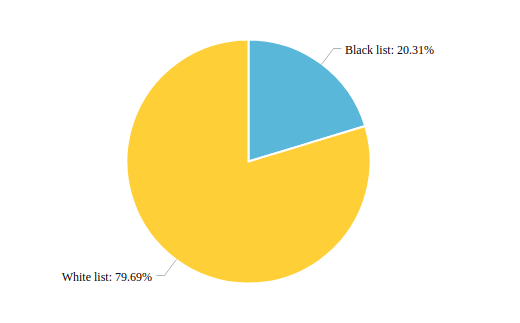
\includegraphics[width=0.7\textwidth]{test_case_1.png}
	\caption{Raportul dintre numarul IP-urilor de pe Blacklist si Whitelist dintr-o luna}
	\label{fig:test_1}
\end{figure}

\begin{figure}
	\centering
	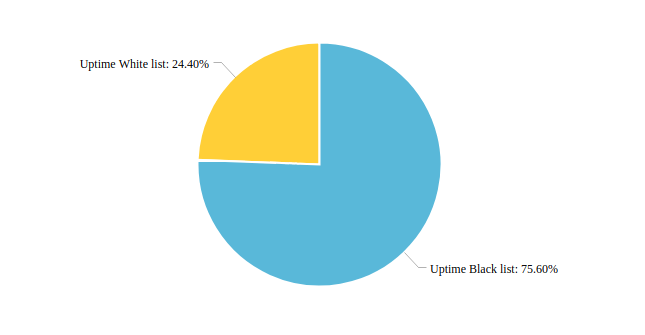
\includegraphics[width=0.7\textwidth]{test_case_2.png}
	\caption{Raportul dintre uptime-ul IP-urile de pe Blacklist si Whitelist din aceasi luna}
	\label{fig:test_2}
\end{figure}


\newpage
%\section{Performance Tests}
 \section{Teste de performanță}

Sitemul propus a fost testat pe doua configuratii diferite pentru PC-ul gazda: Intel Core i7-6600U CPU cu 4 nuclee si o frecventa de 2.6 GHz, cu 16 GB RAM DDR4 si i7-4790k CPU cu 4 nuclee si o frecventa maxima de 4.0 GHz, cu 16 GB RAM DDR4. Ambele sisteme furnizand mult mai multe resure decat cele necesare unei functionari optime. In cea ce priveste resursele minime necesare, acestea trebuie sa fie cele necesare rularii unui sistem de operare Windows 10: un procesor cu o frecventa mai mare de 1.0 GHz si o memorie mai mare sau egala cu 2 GB de RAM. In cea ce priveste capacitatile sistemului de a suporta conexiuni exterioare, acesta nu a fost testat decat manual, prin intermediul unor masini virtuale.